\documentclass[11pt]{article}

\usepackage[a4paper, margin=1in]{geometry}
\usepackage{amsmath}
\usepackage{amssymb}
\usepackage{graphicx}
\usepackage{booktabs}
\usepackage{xcolor}
\usepackage{hyperref}
\usepackage{tikz}
\usepackage{float}
\usepackage{enumitem}
\usetikzlibrary{arrows.meta, positioning}

\hypersetup{colorlinks=true, linkcolor=black, urlcolor=blue}

\title{}
\date{}

\begin{document}

% ================= TITLE PAGE =================
\begin{center}
{\LARGE \bfseries Top 10 AI Algorithms and Techniques Used in Real-World Applications}\\[0.4em]
{\large From Recommendation Systems and Medical Imaging to Generative AI}
\end{center}

\vspace{0.5cm}

\IfFileExists{assets/model_info.png}{
\begin{center}
\includegraphics[width=0.55\textwidth]{assets/model_info.png}
\end{center}
}{}

\vspace{0.3cm}

\begin{center}
\begin{tabular}{ll}
\textbf{Name:} & Devesh \\
\textbf{Roll Number:} & 24111014 \\
\textbf{Department:} & Biomedical Engineering \\
\textbf{Institution:} & NIT Raipur \\
\textbf{Course:} & AI \& ML \\
\textbf{Faculty:} & Prof. Saurabh Gupta \\
\textbf{Date:} & \today \\
\end{tabular}
\end{center}

\vspace{1cm}
\hrule
\vspace{0.5cm}

% ================= INTRODUCTION =================
\section*{Introduction}

There isn't really one single "AI algorithm" that runs everything -- different problems need different tools. Recognising an image, recommending a song, and playing a game all use pretty different approaches. For this assignment I picked ten algorithms/techniques that are actually used in real products today (not just the standard intro-ML list like linear regression or k-means), and for each one I've covered what it is, roughly how it works, one example, and where it's actually used.

\vspace{0.3cm}

% ================= 1 TRANSFORMER =================
\section{Transformer}

The Transformer is the architecture behind most modern language models (GPT, BERT, etc.). Before this came along, models read text word-by-word in order, which was slow. Transformers instead look at the whole sentence at once and figure out which words matter to which other words -- this is called \textit{self-attention}.

Every word gets turned into a Query, a Key, and a Value vector. The model compares each word's Query with every other word's Key to decide how much attention to pay to it:
\[
\operatorname{Attention}(Q,K,V) = \operatorname{softmax}\!\left(\frac{QK^T}{\sqrt{d_k}}\right)V
\]

\begin{figure}[H]
\centering
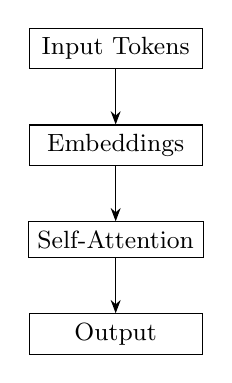
\begin{tikzpicture}[node distance=0.7cm, every node/.style={font=\small}]
\node[draw, minimum width=2.2cm] (a) {Input Tokens};
\node[draw, minimum width=2.2cm, below=of a] (b) {Embeddings};
\node[draw, minimum width=2.2cm, below=of b] (c) {Self-Attention};
\node[draw, minimum width=2.2cm, below=of c] (d) {Output};
\draw[-Stealth] (a)--(b); \draw[-Stealth] (b)--(c); \draw[-Stealth] (c)--(d);
\end{tikzpicture}
\end{figure}

\textbf{Example:} In the sentence "the animal didn't cross the road because it was tired", attention helps the model figure out that "it" refers to the animal, not the road.

\textbf{Used in:} ChatGPT-style language models, translation, code generation, and vision transformers for images.

\textbf{Downside:} needs a LOT of data and compute to train well.

% ================= 2 CNN =================
\section{Convolutional Neural Networks (CNN)}

CNNs are the go-to for image data. Instead of connecting every pixel to every neuron (which would be huge), a small filter slides over the image and picks up patterns like edges, corners, textures.

\[
Y(i,j) = \sum_{m}\sum_{n} X(i+m, j+n)\, K(m,n)
\]

Early layers pick up simple stuff (edges), deeper layers combine those into more complex shapes, and eventually the network can recognise full objects.

\textbf{Example:} classifying a chest X-ray as normal or showing signs of pneumonia.

\textbf{Used in:} medical imaging, face recognition, self-driving car cameras, defect detection on factory lines.

\textbf{Downside:} usually needs a lot of labelled images to train well.

% ================= 3 GNN =================
\section{Graph Neural Networks (GNN)}

Some data isn't a grid or a sentence -- it's a graph. Molecules, social networks, road networks. GNNs work on this kind of data by having each node "talk" to its neighbours and update itself based on what they say. This is called message passing.

\[
h_v^{(l+1)} = \sigma\!\left(W_1 h_v^{(l)} + \sum_{u \in N(v)} W_2\, h_u^{(l)}\right)
\]

\textbf{Example:} predicting whether a new molecule could work as a drug, based on how its atoms are connected.

\textbf{Used in:} drug discovery, fraud detection on transaction networks, some recommendation systems.

\textbf{Downside:} can be tricky to scale to really huge graphs.

% ================= 4 DIFFUSION =================
\section{Diffusion Models}

This is what's behind most AI image generators right now. The training idea is a bit backwards: take a real image, slowly add noise to it until it's just static, and train a model to reverse that -- i.e., remove noise step by step. Once trained, you can start from pure random noise and the model will "denoise" it into a brand new image.

\[
q(x_t \mid x_{t-1}) = \mathcal{N}\!\left(x_t;\ \sqrt{1-\beta_t}\,x_{t-1},\ \beta_t I\right)
\]

(this is the simplified version of the forward noise step -- real systems have a lot more going on, like text conditioning)

\textbf{Example:} typing a prompt like "a cat wearing a spacesuit" and getting a generated image.

\textbf{Used in:} AI image generators, image editing, and some early work in medical image synthesis.

\textbf{Downside:} generating one image takes many steps, so it's slower than a single-pass model.

% ================= 5 RL =================
\section{Reinforcement Learning}

Here the model (called an agent) learns by trial and error instead of from labelled data. It takes an action in an environment, gets a reward (or penalty), and slowly learns a strategy that gets the most reward over time. The tricky part is balancing trying new things (exploration) vs sticking to what already works (exploitation).

\[
Q(s,a) \leftarrow Q(s,a) + \alpha\Big[r + \gamma \max_{a'} Q(s',a') - Q(s,a)\Big]
\]

\textbf{Example:} a robot learning to walk by repeatedly falling over and adjusting.

\textbf{Used in:} robotics, game-playing AI, industrial process control.

\textbf{Downside:} usually needs a huge number of trial-and-error attempts to learn anything good.

% ================= 6 XGBOOST =================
\section{Gradient Boosting / XGBoost}

This one isn't a neural network -- it's an ensemble of decision trees. The idea: train one small tree, see where it messes up, train the next tree to fix those specific mistakes, repeat. XGBoost is just a very fast, optimised version of this idea.

\[
F_m(x) = F_{m-1}(x) + \eta\, h_m(x)
\]

\textbf{Example:} predicting whether a loan applicant is likely to default, based on structured data like income, credit history, etc.

\textbf{Used in:} fraud detection, credit scoring, most "spreadsheet-style" prediction problems in industry.

\textbf{Downside:} not really suited for images or raw text -- works best on structured/tabular data.

% ================= 7 COLLABORATIVE FILTERING =================
\section{Collaborative Filtering}

The basic idea behind a lot of recommendation systems: if two users rated similar things similarly in the past, they'll probably agree in the future too. You build a big user-item matrix (mostly empty, since nobody rates everything) and try to fill in the blanks.

\[
R \approx U V^T
\]

$U$ and $V$ are learned vectors for users and items -- multiplying them gives a predicted rating.

\textbf{Example:} "users who liked this also liked..." on a shopping site.

\textbf{Used in:} platforms like Netflix, Amazon, and Spotify use this alongside other techniques, not on its own.

\textbf{Downside:} doesn't work well for brand new users/items with no history yet (the "cold start" problem).

% ================= 8 CONTENT-BASED / COSINE =================
\section{Content-Based Filtering (Cosine Similarity)}

Instead of looking at what other users liked, this looks at the item itself. A song, for example, could be described as a vector of features like tempo, energy, danceability, etc. Then you just check which songs have similar vectors.

\[
\operatorname{sim}(A,B) = \frac{A \cdot B}{\lVert A \rVert \, \lVert B \rVert}
\]

\textbf{Quick example:} $A=(1,2,3)$, $B=(2,4,6)$. Since $B$ is just $A$ doubled, they point in the exact same direction, so similarity $= 1$ (as similar as it gets).

\textbf{Note:} Spotify doesn't literally just run cosine similarity on a handful of features -- that's an oversimplification. But this kind of vector comparison is a real building block used alongside other methods in music/content recommendation.

\textbf{Used in:} "more like this" recommendations, handling new items with no interaction history yet.

% ================= 9 YOLO =================
\section{YOLO (Object Detection)}

YOLO ("You Only Look Once") is a family of models for detecting objects in images -- not just "what is in this photo" but also "where exactly is it, with a box around it." It does this in one pass over the image, which is what makes it fast enough for real-time video.

\[
IoU = \frac{\text{Area of Intersection}}{\text{Area of Union}}
\]

IoU is just how you measure whether a predicted box actually lines up with the real object.

\textbf{Example:} a self-driving car's camera drawing boxes around pedestrians and other cars in real time.

\textbf{Used in:} self-driving cars, security cameras, traffic monitoring, robotics.

\textbf{Downside:} can miss very small or overlapping objects.

% ================= 10 CONTEXTUAL BANDITS =================
\section{Contextual Bandits}

Kind of a lighter version of reinforcement learning, used a lot in recommendation. Instead of "which item is generally popular," it asks "given this specific user and situation right now, what should I show them?" It picks an action, sees the result (clicked / skipped / etc.), and learns from that -- without worrying about long chains of future decisions like full RL does.

\textbf{Example:} a music app deciding which song to play next based on your recent listening, time of day, etc., and learning from whether you skip it.

\textbf{Used in:} recommendation ranking, online ads, personalised app interfaces.

\textbf{Downside:} doesn't account for how today's decision affects tomorrow's outcome, unlike full RL.


\vspace{15\baselineskip}
% ================= SPOTIFY VECTOR MAP =================
\section{Where This Fits: Spotify's Vector-Based Recommendations}

Since content-based filtering and cosine similarity came up earlier, it's worth looking a bit closer at how Spotify actually uses this kind of idea, since it's a pretty well-known real-world example.

\IfFileExists{assets/spotify_algorithm.png}{
\begin{center}
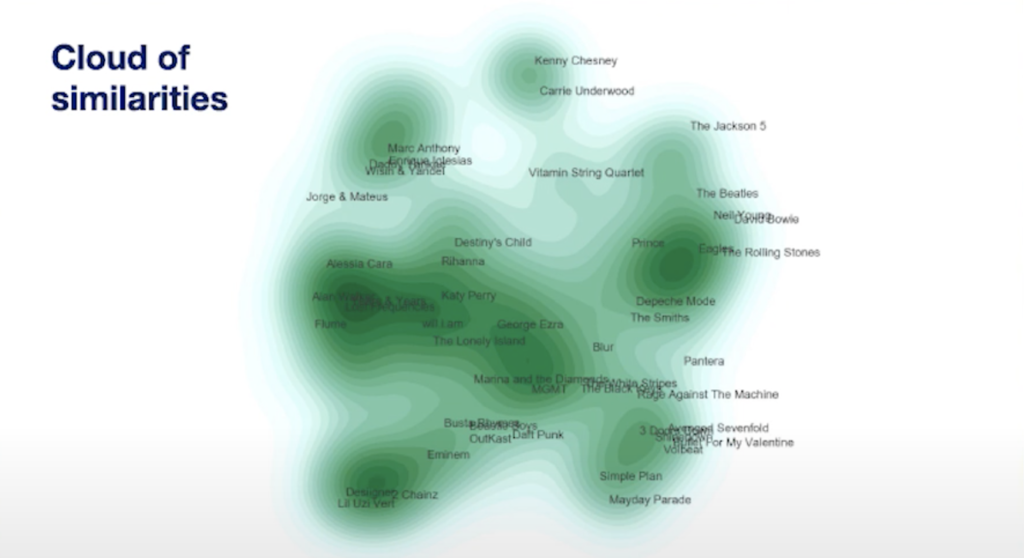
\includegraphics[width=0.7\textwidth]{assets/spotify_algorithm.png}
\end{center}
}{}

The rough idea is that every song (and every user) ends up placed as a point in a large, shared vector space -- sometimes called a "vector map" or embedding space. Songs that sound alike, get listened to together, or show up on the same playlists end up close together in this space, and songs that have nothing to do with each other end up far apart. Once everything is placed like this, recommending a song is basically just finding the nearest neighbours to a point -- which is the same nearest-neighbour/cosine-similarity idea from Section 8, just applied at a much bigger scale.

Where it gets more interesting is \textit{how} the vectors are built. Spotify doesn't only use hand-picked audio features like tempo or energy -- it combines a few different signals into these vectors, roughly:

\begin{itemize}[noitemsep]
    \item audio-based features (rhythm, energy, timbre, etc.)
    \item collaborative filtering signals (which users played/skipped/saved which songs)
    \item NLP-based signals, where songs that show up together in blog posts, playlist titles, or descriptions end up placed closer together
\end{itemize}

So it's really a mix of Sections 7 and 8 (collaborative filtering + content-based similarity) plus some extra text-based signals, all combined into one shared vector space rather than being kept as separate systems.

\textbf{Why this matters:} it's a good example of the point made earlier -- cosine similarity itself is a simple, almost bare-bones formula, but once it's applied to rich vectors built from multiple data sources, it becomes a genuinely powerful recommendation tool.

\textbf{Downside:} the quality of the recommendations is completely dependent on how good the underlying vectors are -- if the embeddings don't capture something meaningful, the "closeness" in the vector space stops meaning much.

% ================= COMPARISON =================
\section{Quick Comparison}

\begin{table}[H]
\centering
\footnotesize
\setlength{\tabcolsep}{3pt}
\begin{tabular}{p{2.2cm} p{2.6cm} p{4.5cm} p{4.5cm}}
\toprule
\textbf{Technique} & \textbf{Data Type} & \textbf{Typical Use} & \textbf{Main Limitation} \\
\midrule
Transformer & Text/sequences & Language models, translation & Very compute-hungry \\
CNN & Images & Medical imaging, vision & Needs lots of labelled data \\
GNN & Graphs & Drug discovery, networks & Hard to scale to huge graphs \\
Diffusion & Images/audio & AI image generation & Slow to generate \\
RL & Sequential decisions & Robotics, games & Needs tons of trial and error \\
XGBoost & Tabular data & Fraud, credit risk & Bad for images/raw text \\
Collaborative Filtering & User-item ratings & Recommendations & Cold-start problem \\
Content-Based (Cosine) & Feature vectors & Similar-item recommendations & Depends on good features \\
YOLO & Images & Object detection & Struggles with tiny objects \\
Contextual Bandits & Context + reward & Personalisation, ads & Ignores long-term effects \\
\bottomrule
\end{tabular}
\end{table}

There's no single "best" one here -- it really depends on the type of data you have, how much compute you can throw at it, and what the actual problem is.

% ================= COMBINING =================
\section{They're Usually Combined, Not Used Alone}

One thing that stood out while researching this: real products almost never rely on just one of these. A recommendation system, for example, might use collaborative filtering to shortlist candidates, content-based similarity to catch new items, a neural net to build embeddings, and a ranking model to decide the final order. So even something as "simple" as cosine similarity can be a small but useful piece of a much bigger pipeline.

% ================= CONCLUSION =================
\section{Conclusion}

These ten techniques cover a pretty wide range of AI -- language, vision, graphs, recommendations, and decision-making. What's interesting is that AI these days is less about one clever formula and more about combining several of these tools, good data, and user feedback into something that actually works in practice.

\end{document}
